% Spellchecking done with grammarly
\chapter{Background and Related Work}
As mentioned in the introduction, the high computational cost of principal component analysis introduces a significant challenge for real-time anomaly detection, especially as the volume of data grows really large. To address this limitation, \parencite[p.~1]{rakuschek2025visual} proposed combining time delay embedding (TDE) with principal component analysis (PCA). His final implementation generates visual plots from vibration data that resemble human fingerprints. This chapter explains the theoretical foundations of principal component analysis and time delay embedding in detail, identifies key computational bottlenecks, and reviews the original offline implementation of the algorithm.

% Spellchecking done with grammarly
\section{Baseline Methodology}
The purpose of the underlying paper was to create an algorithm which solves the issue of plotting vibration data on a line graph where the observer can't distinguish between noise and the actual vibrations. The overall goal was to: further enhance and complement the visual inspection in the time
domain, enabling users to quickly gain an overview of different
vibration profiles within the signal or to detect periodicity within
noise. (\cite{rakuschek2025visual} p.1). In the background this was done by using  time delay embeddings, which is a method that takes the time series data and transforms it into a point cloud which can than be projected onto a 2D plane. Another really important aspect of the algorithm which is to be transformed is the use of principal component analysis. It is a dimensionality reduction technique that helps reduce the number of features in a dataset while keeping the most important information. As stated by \textcite{KarlPearson}, principal component analysis simplifies complex datasets by transforming correlated features into a smaller set of uncorrelated components. When the two algorithms are applied on a harmonic oscillation the result is a ellipsoid and as more noise is added its really hard to distinguished between noise or the hidden signal. However, applying time delay embedding with appropriate window sizes effectively reveals the underlying vibration signal.

% Spellchecking done with grammarly
{\section{Concepts}}

In the following paragraphs the offline  algorithm by \cite{rakuschek2025visual} is explained in more detail. Additionally the  main underlying mathematical methods, namely PCA,TDE and sliding Windows are discussed. Finally an overview over the related work is provided.

\subsection{Time delay Embeddings}
Time Delay Embedding (TDE) creates a multidimensional geometrical object from a single time series signal. Given a scalar signal $x(t)$, where $x(t) \in {R}$ represents any measurement at time $t$, standard one dimensional analysis often fails to reveal underlying structural properties. In contrast, the embedding transforms the temporal signal to a multidimensional space, revealing underlying attractors, trajectories, and regime changes. This turns the dynamic temporal problem into a geometric problem which is significantly easier to solve. Under optimal operating conditions, the signal traces clear, predictable geometric shapes (such as ellipsoids, straight lines or circles), making normal behavior easy to distinguish from anomalies. The embedded state vector $X(t)$ is constructed as:
$$X(t) = [x(t), x(t - \tau), x(t - 2\tau), \dots, x(t - (d - 1)\tau)]$$
where $x(t)$ represents the continuous signal at time $t$, $d$ denotes the embedding dimension, and $\tau$ is the time delay. 
For discrete time series data $x = [x_1, x_2, x_3, \dots, x_N]$, choosing $d = 3$ and $\tau = 1$ transforms the sequence $[x_1, x_2, x_3, x_4, x_5]$ into the following set of 3D points:
$$[x_1, x_2, x_3], \quad [x_2, x_3, x_4], \quad [x_3, x_4, x_5]$$
The embedding dimension $d$ defines how many past samples are used to reconstruct the state. If the parameter $d$ is chosen too small, the dynamics are not fully shown; if chosen too large, the noise is amplified. The delay $\tau$ defines the spacing between the samples. \\
Periodic machine vibrations naturally map to elliptical structures, this geometric behavior is the result of plotting a harmonic signals $x(t)$ against its time delayed counterpart $x(t - \tau)$ which forms a two dimensional phase plot, where periodic oscillations trace a closed elliptical trajectory. In contrast random uncorrelated noise forms a scattered cloud.
As stated by \textcite[p.~4]{rakuschek2025visual}, TDEs serve as an effective fingerprinting technique for vibration signals, enabling clear visual identification of changes in vibration profiles and underlying periodicity.
\subsection{Principal Component Analysis}

Principal component analysis is a dimensionality reduction technique that transforms high-dimensional correlated data into a smaller set of uncorrelated variables.
The algorithms task is to handle the high dimensional vector spaces generated by time delay embeddings. Rather than operating on the raw multi variable data directly, principal component analysis takes the d-dimensional embedding vectors into an orthogonal coordinate system. The method identifies the directions of maximum variance (the principle components), thereby compressing the high dimensional space trajectories into a lower-dimensional subspace, most commonly two dimensions, while preserving the dominant dynamic characteristics of the vibration signal.
\label{section:foundation}
\subsection{Foundation}
Plotting the raw TDE output yields a point cloud with a complex geometry in $d$-dimensional space. This point cloud is characterized by two main properties: directions of maximum variance and their corresponding magnitudes. The directions give the orientation in space where the data varies, and the magnitudes tell how much the data spreads in each direction. The directions where the data varies the most are exactly where the information lies; on the other hand, noise can be found where very little variation is present.
\begin{figure}[H]
\centering
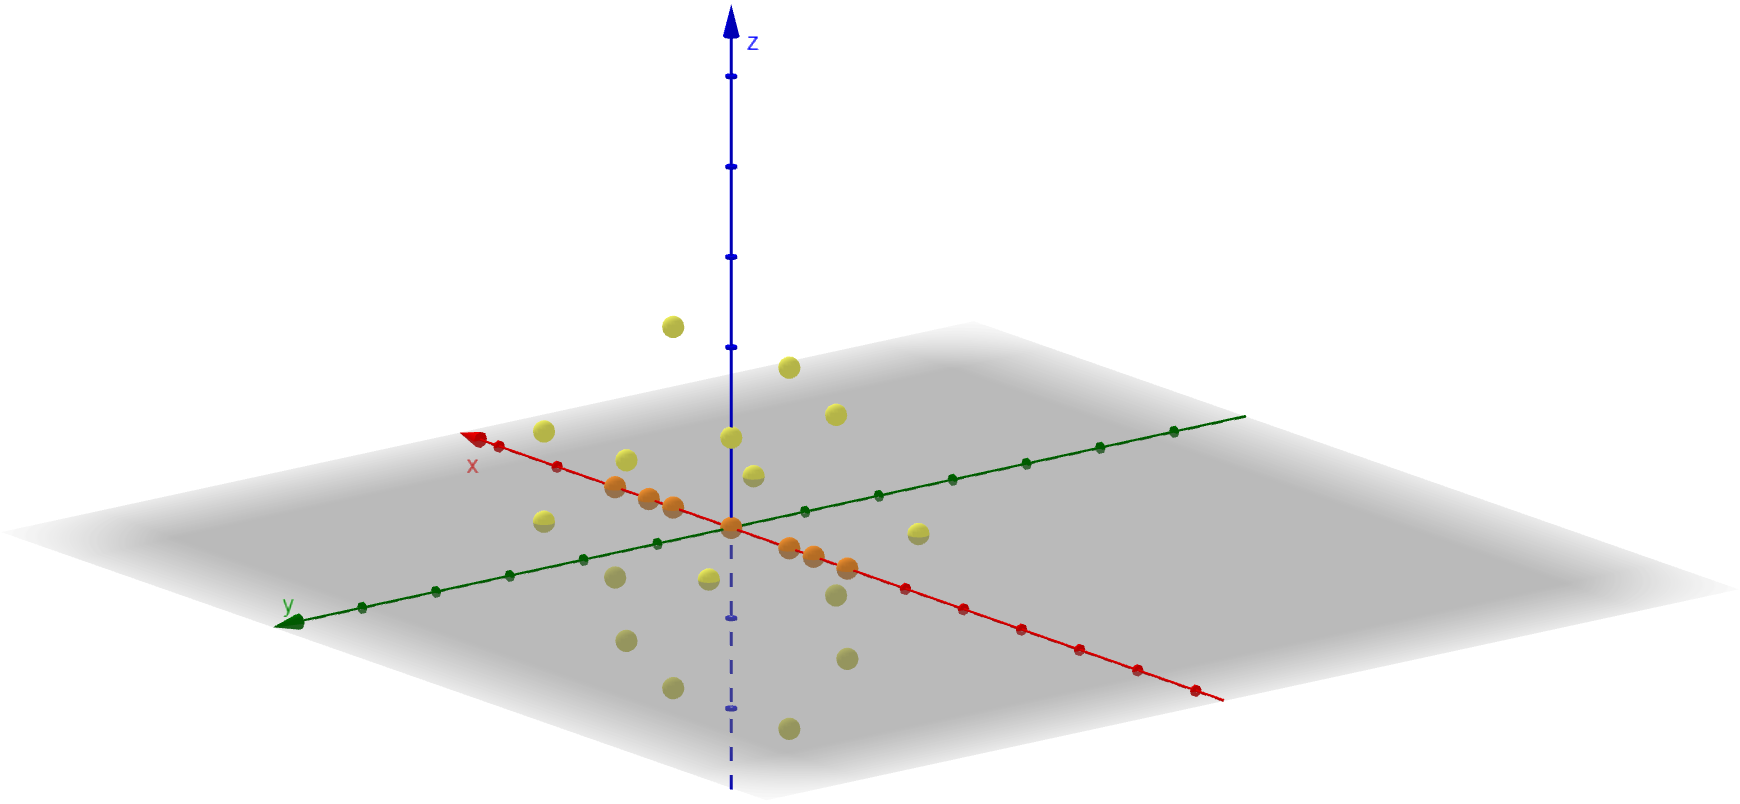
\includegraphics[width=0.7\textwidth]{figures/3dPointcloud.png}
\caption{Visualization of a 3D phase-space point cloud (yellow) and its 1D projection along the principal axis of maximum variance (orange).}
\label{fig:pointCloud}
\end{figure}
One possible approach would be to project all these points onto one single dimension. However, as visualized in Figure~\ref{fig:pointCloud}, when projecting all points onto a single axis, all additional data is lost(demonstrated by the orange points).
When a point $\mathbf{x}$ is projected onto a unit vector $\hat{\mathbf{u}}$, the resulting projected vector $\mathbf{x}'$ lies along $\hat{\mathbf{u}}$ with a magnitude defined by the inner product $\mathbf{x}^T \hat{\mathbf{u}}$:
\begin{equation}
\mathbf{x}' = (\mathbf{x}^T \hat{\mathbf{u}}) \hat{\mathbf{u}}
\end{equation}
The squared inner product $(\mathbf{x}^T \hat{\mathbf{u}})^2$ represents the magnitude of the projection. This squared quantity is minimized when $\mathbf{x}$ is orthogonal to $\hat{\mathbf{u}}$ and maximized when $\mathbf{x}$ is parallel to it. 

The method tries to find the unit vector $\hat{\mathbf{u}}$ that maximizes the sum of these squared projections across the entire dataset. Using the sample covariance matrix
\begin{equation}
\mathbf{C} = \frac{1}{N} \sum_{i=1}^{N} \mathbf{x}_i \mathbf{x}_i^T
\label{eq:covariance_matrix}
\end{equation}
the variance of the projected data is given by $\hat{\mathbf{u}}^T \mathbf{C} \hat{\mathbf{u}}$. Maximizing this variance subject to the constraint $\hat{\mathbf{u}}^T \hat{\mathbf{u}} = 1$ leads to the eigenvalue equation:
\begin{equation}
\mathbf{C}\hat{\mathbf{u}} = \lambda\hat{\mathbf{u}}
\label{eq:eigenvalue_equation}
\end{equation}
This proves that the principal directions of the data correspond to the eigenvectors of the covariance matrix $\mathbf{C}$. Since the variance along any given principal axis equals its corresponding eigenvalue $\lambda$, the eigenvector associated with the largest eigenvalue is the optimal direction that preserves the maximum amount of information.
\subsection{Computation}
Prior to computing the covariance matrix, the dataset has to be centered. This step is a mandatory preprocessing step in principal component analysis to ensure that the origin of the coordinate system matches with the sample mean $\boldsymbol{\mu}$. Without centering, the first principal component would reflect the shift of the dataset relative to the origin rather than displaying the directions of maximum variance. Here, the mean vector is defined by:
\begin{equation}
\boldsymbol{\mu} = \frac{1}{N} \sum_{i=1}^{N} \mathbf{x}_i
\label{eq:mean_vector}
\end{equation}
Following this, the centered vector $\tilde{\mathbf{x}}_i$ for each data point is defined as:
\begin{equation}
\tilde{\mathbf{x}}_i = \mathbf{x}_i - \boldsymbol{\mu}
\label{eq:centering_vector}
\end{equation}
Where $X$ is the current window mean. 
The covariance matrix $S$is then computed as:
\begin{equation}
\mathbf{S} = \frac{1}{n-1} \tilde{\mathbf{X}}^T \tilde{\mathbf{X}}
\end{equation}
The resulting covariance matrix $C$ quantifies how each pair of embedded variables varies together. By performing an eigen decomposition of the covariance matrix it gives back its eigenvalues $\lambda_1 ,\lambda_2....\lambda_d$ and corresponding eigenvectors $\mathbf{u}_1, \mathbf{u}_2, \dots, \mathbf{u}_d$, where each one of the eigenvalues $\lambda$ represents the variance captured along its its associated principal component\parencite[p.~382]{rencher2002methods}.
The resulting principal components scores represent the transformed data coordinates in the new orthogonal space are calculated by projecting the centered time delay embedding data matrix $\tilde{X}$ onto the matrix of eigenvectors $\mathbf{U} = [\mathbf{u}_1, \mathbf{u}_2, \dots, \mathbf{u}_d]$:
\begin{equation}
\mathbf{Z} = \tilde{\mathbf{X}}\mathbf{U}
\label{eq:pca_scores}
\end{equation}
Here, $\mathbf{Z} \in {R}^{N \times d}$ contains the projected principal component scores, where each column $i$ corresponds to the projection along the $i$-th eigenvector $\mathbf{u}_i$ where $\mathbf{U}$ denotes the matrix of extracted eigenvectors. For this specific area of application only the first two principal components $z_1$ and $z_2$ are kept. These components capture the most of the variance in the system while reducing the data from any $d$ down to two dimensions, which is easier to plot. Combining time delay embedding  with principal component analysis is especially effective in this use case because time delay embedding reconstructs the system dynamics in phase space, while principal component analysis is able to identify the lower-dimensional projection that preserves maximum variance, thereby making structural anomalies more visible. 
Only the first two principal components are kept as these components explain the major variance in the data. This allows a wide range of applications not only to anomaly detection but also to broader domain tasks requiring information preserving dimensionality reduction like image or data compression.



\subsection{Original source code}
\label{section:OriginalImplementation}
\textcite{rakuschek2025visual} offline implementation was written in Python and focuses on two core functions. \\
A time delay embedding function takes an 1D input signal (as a NumPy array) and the parameters $d$ (embedding dimension), $\tau$ (time delay), and $s$ (stride or window step size). By default tau and stride is set to one. The function uses a multidimensional array to store the individual windows of length $d$. The tau enforces the step size between the elements in each window, a larger value spreads the window further apart in time.
The stride determines how many samples to move forward before creating the next window, a larger stride produces fewer output points.
As shown in the supplemental material \textcite{Supplemental_document}, larger values for $\tau$ and s result in a thinner point cloud while the overall circular structure remains. \\
The plotting function takes an subplot, the multidimensional array resulting from the time delay embedding function and an title, which is per default "TDE", as parameters.
For the principal component analysis, the scikit-learn python library was used, the function essentially reduces the given time delay embedding output from its $d$ to two dimensions. In the next step, the scores which are the distances of each point from the origin are calculated, these euclidean distances from the origin are normalized to the range [0, 1] and the points are plotted with colors mapped to their normalized distances.
\subsection{Visual comparison}
Conventional time series representations of vibration signals and highly clustered data in general tend to suffer from over-plotted when high-frequency noise is observed over a extended time period. As shown in Figure \ref{fig:BadExample}, high sampling rates compress the signal into an high-density amplitude block. The result is that phase shifts and harmonic distortions remain visually hidden consequently making it unsuitable for condition monitoring. 
\begin{figure}[H]
\centering
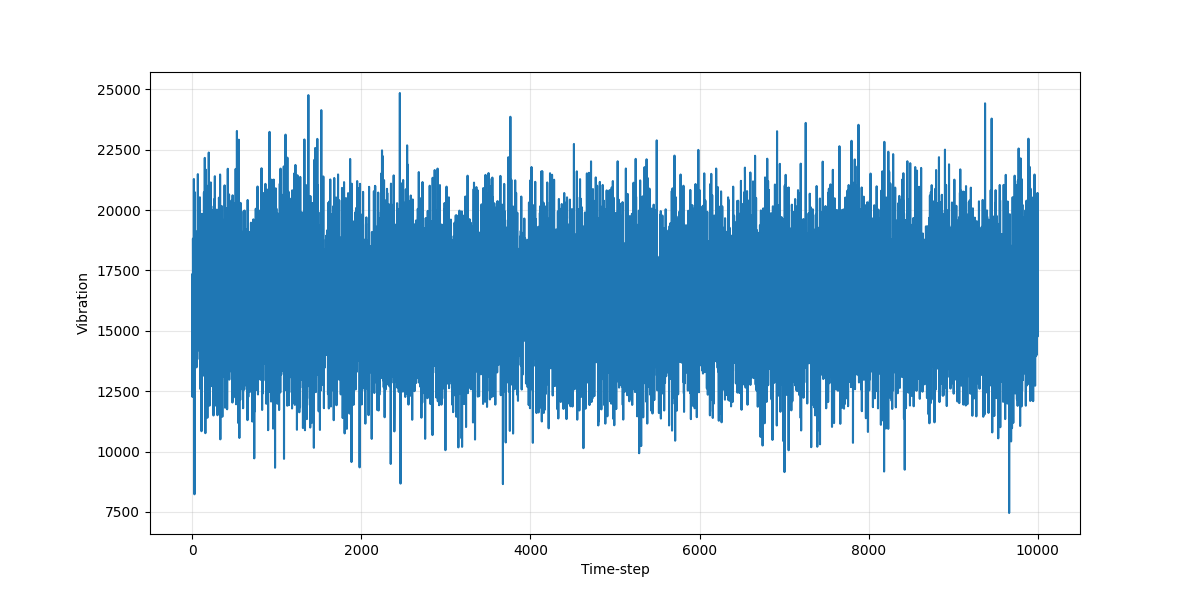
\includegraphics[width=0.7\textwidth]{figures/vibration_data.png}
\caption{Example of the raw vibration signal.}
\label{fig:BadExample}
\end{figure}
In contrast, transforming the data into a Time Delay Embedding phase space produces a highly compact visually informative fingerprint.Figure \ref{fig:tdeHealty} shows the baseline fingerprint under healthy normal operating conditions, generated with the algorithm described in Section \ref{section:OriginalImplementation} 
A healthy fingerprint is characterized by signal periodicity, which "results in elliptical structures and 'round' point cloud shapes" \cite{rakuschek2025visual}. Furthermore, "noise accumulates near the center while vibrations cause the circular patterns with a larger radius than noise," with these circular structures persisting even under high noise levels \cite{rakuschek2025visual}.
\begin{figure}[H]
\centering
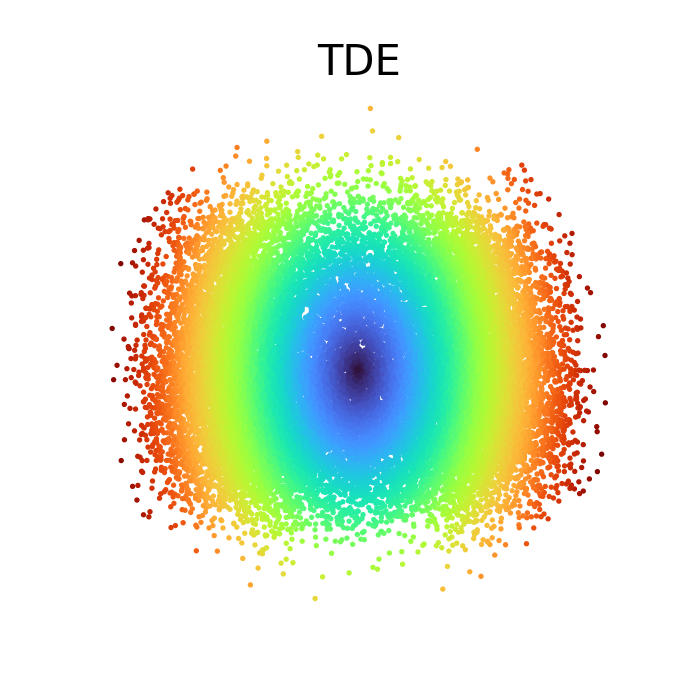
\includegraphics[width=0.5\textwidth]{figures/tdeVisual.png}
\caption{Example of a faulty fingerprint from a machine running in presence of mechanical imbalance at shaft.}
\label{fig:tdeBadExample}
\end{figure}
\begin{figure}[H]
\centering
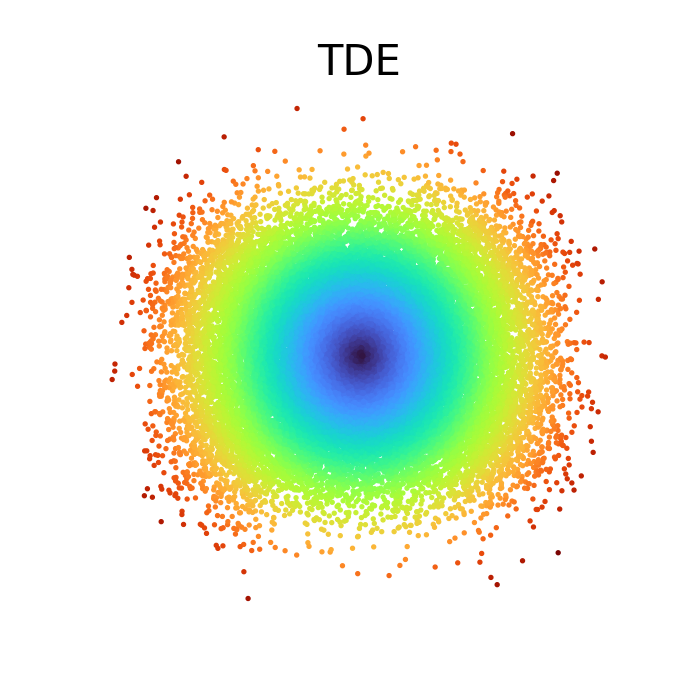
\includegraphics[width=0.5\textwidth]{figures/healtyFingerprint.png}
\caption{Example of a fingerprint under no faulty conditions.}
\label{fig:tdeHealty}
\end{figure}
Comparing the faulty fingerprint in Figure\ref{fig:tdeBadExample} with the healthy baseline in Figure \ref{fig:tdeHealty} shows distinct geometric distortions. For instance in figure \ref{fig:BadExample} a mechanical shaft imbalance wraps the phase trajectory into an asymmetric pattern while the healthy fingerprint shows a clean and periodic shape. 


\section{Related work}
\subsection{Incremental principal component analysis}
Conventional Principal component analysis requires storing all observations made over time and calculating full matrix eignedecomposition, introducing a high computational complexity which is unsuitable for real time anomaly detection. A smart solution is to shift the computational load to functions which are able to reuse already calculated values for its computation lowering the computational cost massively.Following the incremental principal component analysis framework introduced by \textcite{Incremental_PCA}, the proposed pipeline maintains running data statistics and updates the dominant eigenspace iteratively upon receiving each new observation.
Even with this optimization steps a central challenge remains: extracting the eigenvectors of the covariance matrix at every iteration step.  
According to \textcite[p.~2931]{1468483}, note that traditional signal subspace estimation relies on eigenvalue or singular value decomposition, whose inherent computational complexity creates a genuine need for fast subspace tracking techniques in adaptive signal processing. This motivates the subspace tracking approach, which instead avoids full eignedecomposition by iteratively refining an estimate of the dominant eigenvectors.
\subsection{Subspace tracking}
One problem that arises when working with principal component analysis is that the result, which is an covariance matrix, is often of higher dimension and computationally challenging to diagonalize directly via a full eignedecomposition. The subspace iteration method solves this issue by iteratively estimating the dominant eigenvectors instead of solving the eigenproblem at each iteration step. \textcite[p.~270]{Oja1982SimplifiedNM} proves that a simple Hebbian-type update rule combined with normalization converges with probability one to the dominant eigenvector of the input correlation matrix, provided the largest eigenvalue has multiplicity one. This provides the theoretical basis for implementing the subspace iteration method to solve the eigenvector problem.
Following this principle the eigenvector solver used in the principal component analysis routine follows the classical power iteration scheme described by \textcite[p.~2932]{1468483}, which alternates a data compression step—multiplying the correlation matrix by the current subspace estimate—with an orthonormalization step at each iteration.
However \textcite[p.~2932]{1468483} points out that the classical power iteration method is unsuitable for real-time processing due to its computational cost, which scales with the ambient dimension $n$ of the data; this motivated the development of faster approximations such as API and FAPI. 
To achieve fast convergence requires the covariance matrix to be kept as small as possible. Since in this thesis the covariance matrix is computed over the $d$-dimensional embedding space rather than on an large continuous array, the power iteration remains computationally stable for real time use without requiring these approximations.


\subsection{Phase Space Reconstruction and time delay embedding}
As summarized by \textcite{Tan_2023}, the embedding theorem guarantees that, 
\subsection{Sliding Window}
The sliding window approach is a method for processing steaming data using a fixed -size buffer that retains only the most recent observations. As new data arrives, older data points are discarded while more recent data points are continuously appended to the  buffer. \\ In the context of this thesis, the sliding window approach is applied to the time series data before the Time delay Embedding (Section 2.2.1) and Principal Component Analysis (Section 2.2.2). This fulfills the key requirement of handling steaming data efficiently while maintaining constant memory usage  and low latency.  \\
According (\cite{https://doi.org/10.1155/2014/879736} p.14 ), given a time series $T$ of length $m$ and a user-defined subsequence length $n$, all possible subsequences $C_p$ can be extracted by sliding a window of size $n$ across $T$.
This formalization reflects how sliding window mechanism extracts sequential segments from continuous time-series data.
\subsection{Industrial vibration monitoring solutions}
Two of the most established innovators in the field od real-time machine monitoring are Bently Nevada and Emerson, which offer a wide range of wireless and hardwired solutions along with corresponding data visualization. Their customers come from large-scale industries sectors such as power generation, mining and steel production. However the visualization provided typically remains limited to raw amplitude plots, which require high domain expertise and do not offer a an intuitive overview of machine health. 
\begin{figure}[H]
\centering
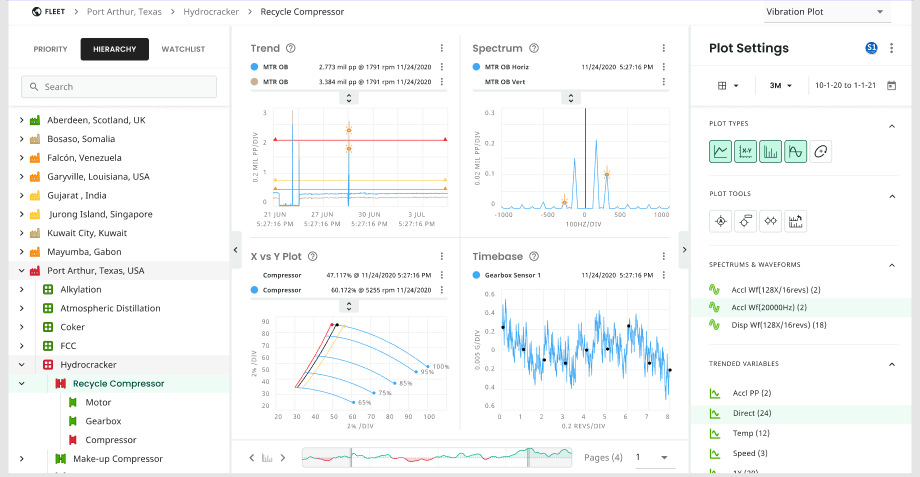
\includegraphics[width=0.8\textwidth]{figures/test2.png}
\caption{Dashboard example from a commercial condition-monitoring platform.\parencite{snyder2021roadmap}}
\label{fig:dashboardBentlyNevada}
\end{figure}
It must be pointed out that the data shown in figure \ref{fig:dashboardBentlyNevada} does not represent sensible customer data but rather only plots mock data for demonstration purposes provided by the vendor.
The dashboard provides an example offered by such platforms: \textcite{snyder2021roadmap} a full complement of diagnostic plots is provided, including polar, orbit, waveform, spectrum, waterfall, air gap, X-Y, multivariable trend, bode and amplitude phase time, and others. While this offers comprehensive coverage, no plot is designed ti make periodic behavior immediately visible at first sight. In contrast the system requires to interpret a specific aspect of the signal separately. A fingerprint plot such as the ones produced by principal component analysis would be a valuable extension to the already established workflows offering a better overview of periodicity and structural changes that normally would require cross referencing across multiple specialized plots.
